\documentclass[11pt, letterpaper, twocolumn]{article}

% Input
\usepackage[english]{babel}
\usepackage[utf8]{inputenc}
% Geometry
\usepackage[margin=1.0in]{geometry}
\usepackage{titlesec}
\titleformat*{\section}{\large\bfseries}
% Fonts
%\usepackage{fontspec}
%xs\setmainfont{Arial}
% Figures and Symbols
\usepackage{graphicx}
\usepackage{caption}
\captionsetup[figure]{font=small}
\usepackage{amsmath}
\usepackage{amssymb}
\usepackage[]{siunitx}
% Misc
\usepackage{epigraph}
% Fancy Header
\usepackage{fancyhdr}
\setlength{\headheight}{14.5pt}
\pagestyle{fancy}
\fancyhf{}
% \renewcommand{\headrulewidth}{0pt}

\lhead{Fluid Simulation in Computergraphics} 
\rhead{Group 4: Ertural, Ledwon} 
\rfoot{\thepage}


\begin{document}
% Title, Abstract
\twocolumn[
\begin{@twocolumnfalse}
  \begin{center}
    \textbf{Fluidsimulation in Computergraphics:
      \\Weakly Compressible Smoothed Particle Hydrodynamics
      \\and Position Based Fluids}
  \end{center}
  \begin{abstract}
    
  \end{abstract}
  \end{@twocolumnfalse}
]


\section*{Introduction} \label{sec:introduction}

\epigraph{Reading maketh a full man; conference a ready man; and writing an exact man.}
{\textit{Sir Francis Bacon}}

% background information
% jargon
% relevant reviews, papers, studies

\section*{Methods} \label{sec:methods}

In the following section we will give an overview of our implementation of a fluidsolver based on the SPH and PBF frameworks.
We will take a look at the general structure of the implementation and discuss specific parts that are different from the given assignment.
For a thorough discussion of the SPH and PBF framework we refer the reader to the review of SPH fluids by Ihmsen et al. \cite{ihmsen2014} and to the original paper about position based fluids by Macklin et al. \cite{macklin2013}.

The implementation uses a C-style imperative approach with the exception of a few object oriented paradigms. Data encapsulation in the form of C++ classes is applied to ensure data consistency during computation. Basic inheritance is used to be able to reuse code for different parts of the program. This style of programming allows us to be flexible enough to incrementially implement the practical assignment tasks while sacrificing little to no performance due to design overload.  

The implementation is divided into three general categories. The solvers, the emitter and particlesystems and the category of auxilary functions. A particlesystem is a collection of particles which are represented by basic attributes, such as mass, density, position, velocity and the accumulated external forces on the particles. Since it is vital to keep all attributes of a particlesystem consistent during computation a particlesystem object is only allowed to be created by the emitter object. The emitter object is a singleton, which means that there is always one and only one single instance of the object during the runtime of the program. During runtime a particlesystem is present in two forms, either as fluid particles or as boundary particles. These subtypes posess attributes and methods responsible for the behaviour of fluid or boundary particles in a system. For example, boundary particles possess a seperate variable volume attribute and a method to compute the volume for each particle depending on the density, e.g. the number of boundary particles in close neighbourhood.

Boundary particles are used to realise the interaction between the fluid and rigid boundaries. As boundaries in a scene are usually represented by triangular mesh models, we create a boundary particlesystem by sampling each triangle of a given input mesh. To this end, it is reasonable to dissolve a higher resolution mesh into a low resolution mesh which still contains the shape information and use this low resoltion mesh for the simulation and keep the original high resolution mesh for rendering the final simulation. This will reduce the overall number of triangles and therefore the number of sampled particles.

\begin{figure}[ht]
    \centering
    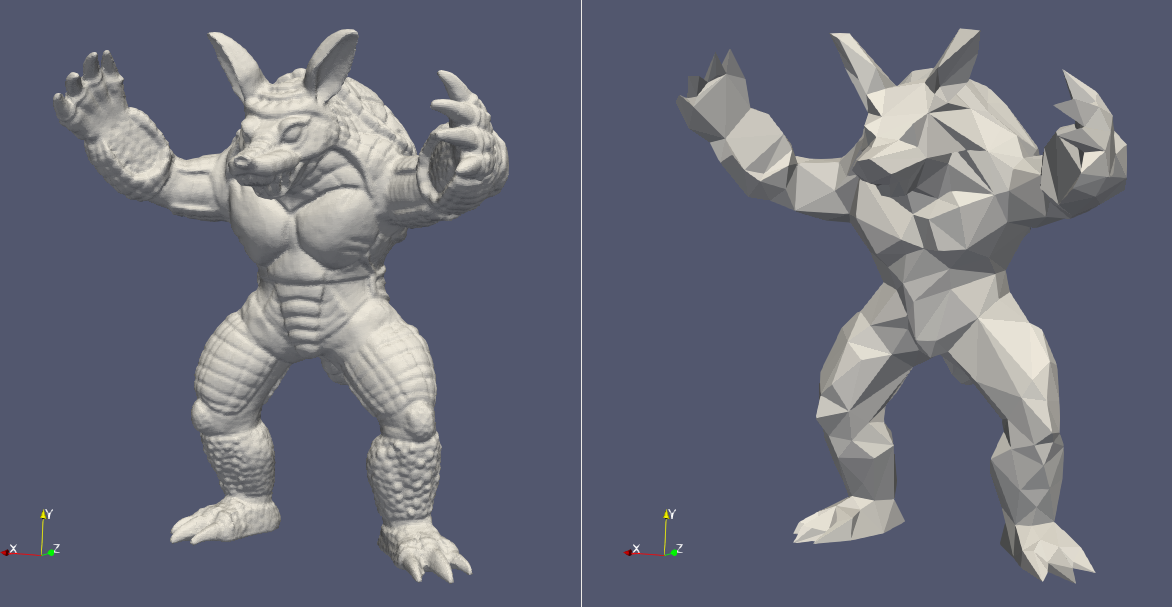
\includegraphics[width=0.5\textwidth]{images/mesh.png}
    \caption{High resoltuion mesh for rendering (left) and low resolution mesh for simulation (right). The mesh on the left maintains the qualitative shape of the mesh.}
    \label{fig:mesh}
\end{figure}


To sample the particles on a triangle surface we perform a variation of the Pineda algorithm \cite{pineda1988} in the local coordinate system of the triangle surface. Given a triangle specified by the three vertex points \(a, b, c \in \mathbb{R}^3\), we construct the orthonormal base vectors \(u,v,n \in \mathbb{R}^3\) defining the triangle surface. The basis transform that will yield the local triangle coordiantes \(p \in \mathbb{R^2}\) for a point in global space \(x \in \mathbb{R}^3\) is given in equation \ref{eq:localtriangle}.

\begin{equation}
  p = 
  \begin{pmatrix}
    u_x & u_v & u_z & u^T a\\
    v_x & v_v & v_z & v^T a\\
    0 & 0 & 0 & 1 \\
  \end{pmatrix}
  \cdot x 
\label{eq:localtriangle}
\end{equation}

Note that the projected point is in homogeneous two dimensional space, as we are only interested in sampling the surface of the triangle. Applying the pineda algorithm is now straight forward. We first enclose the triangle by a bounding box by determining the minimal and maximal coordinates in the projected space. We then go along the bounding box and check for each sample point if its inside the triangle by checking against its edges, as described by Pineda \cite{pineda1988}. We use a hexagonal sampling pattern to ensure maximum coverage of the surface. Figure \ref{fig:trianglesampling} demonstrates the hexagonal sampling in the bounds of the rectangle enclosing the triangle in its local coordinate system. Note that sample points that slightly touch the border are also taken to be in the surface of the triangle. This is achieved by allowing an offset of the particle radius and is used to ensure that the triangle mesh of the boundary has no holes where the edges of two triangles meet. The oversampling is later compensated by recomputing the volume of each sample depending on the number of samples in its close neighbourhood.

\begin{figure}[ht]
    \centering
    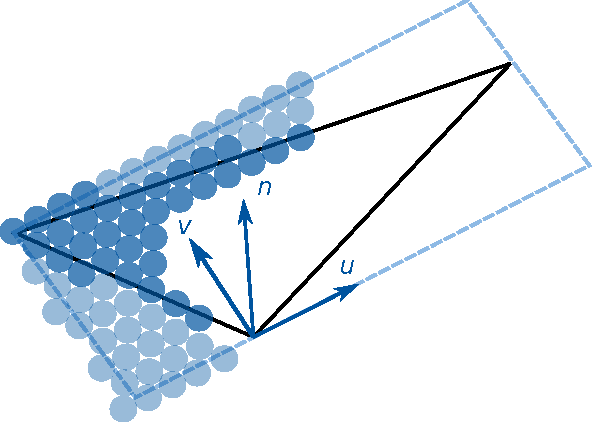
\includegraphics[width=0.5\textwidth]{images/triangle.pdf}
    \caption{Hexagonal sampling using pineda algorithm in local triangle space.}
    \label{fig:trianglesampling}
\end{figure}

Given the sample points computed in the two dimensional surface plane, we transform the points back into three dimensional global space by multiplying them by the inverse of the matrix given in equation \ref{eq:localtriangle}. Since the matrix is orthonormal its inverse is given by simply transposing the matrix.


The boundary particle radius should optimally be the same as the fluid particle radius. This is due to the timestep being determined by the Courant-Friedrich-Levy (CFL) condition, e.g. \( \Delta t \leq \lambda \frac{h}{v^{max}}\) which dictates, that a particle moves a maximum distance of its own radius \(h\) per time-stamp \(\Delta t \). If the boundary particle radius is much smaller. The fluid particles may tunnel through the boundary if the timestep is too high. If the boundaryparticle radius is too high, the boundary shape information is lost and the interaction therefore incorrect. The constant factor \(\lambda\) in the CFL is set around 0.4 in all further simulations.



% demonstrate scientific reasonng
% what were the confounding factors? how did we overcame them?


\section*{Results}
\label{sec:results}


\section*{Conclusion}
\label{sec:conclusion}

% respong to introduction and discuss implications of result


\section*{Outlook}
\label{sec:future}

% what are the next steps?
% what did we learn from this and how could we apply this for the future?


\bibliographystyle{ieeetr}
{\footnotesize
\bibliography{references.bib}}


% tables, if needed, are like this.
% \begin{table}[ht]
% \begin{tabular}{|l|l|l|}
% \hline
% Time (s) & Distance (m) & Charge (C) \\ \hline
% 0        & 0            & 10         \\ \hline
% 1        & 1            & 5          \\ \hline
% 2        & 4            & 6          \\ \hline
% \end{tabular}
% \caption{An example table.}
% \label{table:ExampleTable}
% \end{table}

% \begin{figure}[ht]
%     \centering
%     \includegraphics[width=0.5\textwidth]{img/generic_plot.pdf}
%     \caption{Here is a caption for a figure.}
%     \label{fig:ExampleFigure}
% \end{figure}

\end{document}

%%% Local Variables:
%%% mode: latex
%%% TeX-master: t
%%% End:
